\newpage
\chapter{Инсталация и стартиране}
\label{chapter01}

Софтуерният продукт Calc е част от пакета Apache OpenOffice. Пакетът първоначално е известен с названието StarOffice и е разработен като комерсиален софтуер от немската компания Star Division (от 1985 година). През 1999 година компанията Sun Microsystems изкупува Star Division и през 2000 година Sun публикуват кода на продукта, под отворен лиценз и с променено име – OpenOffice.org. Целта на компанията е да предложи алтернатива на комерсиалният Microsoft Office пакет. През 2010 Oracle Corporation изкупува Sun Microsystems, но продуктът не получава очакваното внимание. Поради стриктно комерсиалната линия водена от Oracle, продуктът е клониран под названието LibreOffice през 2011 година. През същата година Oracle променят лиценза на основния продукт и го предлагат през Apache Software Foundation. 

\section{Сваляне и инсталация}

Продуктът е достъпен от основната си уеб страница на URL адрес (Фиг. \ref{figure0001}): https://www.openoffice.org/download/

\begin{figure}[h!]
  \centering
  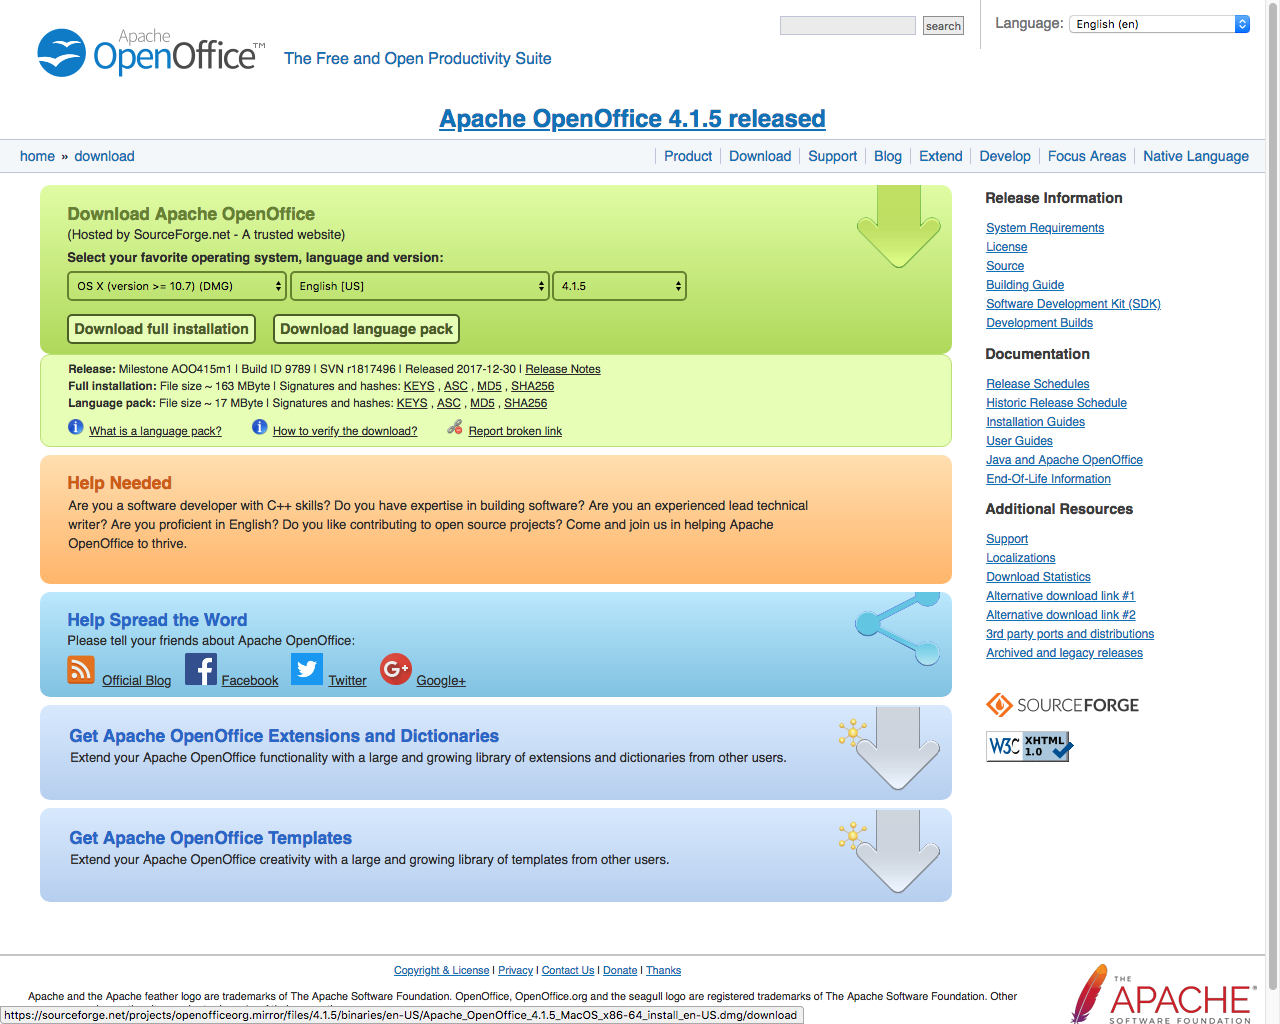
\includegraphics[width=1.0\linewidth]{pic0001}
  \caption{Страница за сваляне на OpenOffice}
\label{figure0001}
\end{figure}
\FloatBarrier

На страницата за сваляне\index{сваляне на продукта} на продукта потребителят трябва да избере вида на операционната си система, основният език на който ще бъде потребителския интерфейс и версията, която желае да инсталира на локалната си машина. 

\begin{figure}[h!]
  \centering
  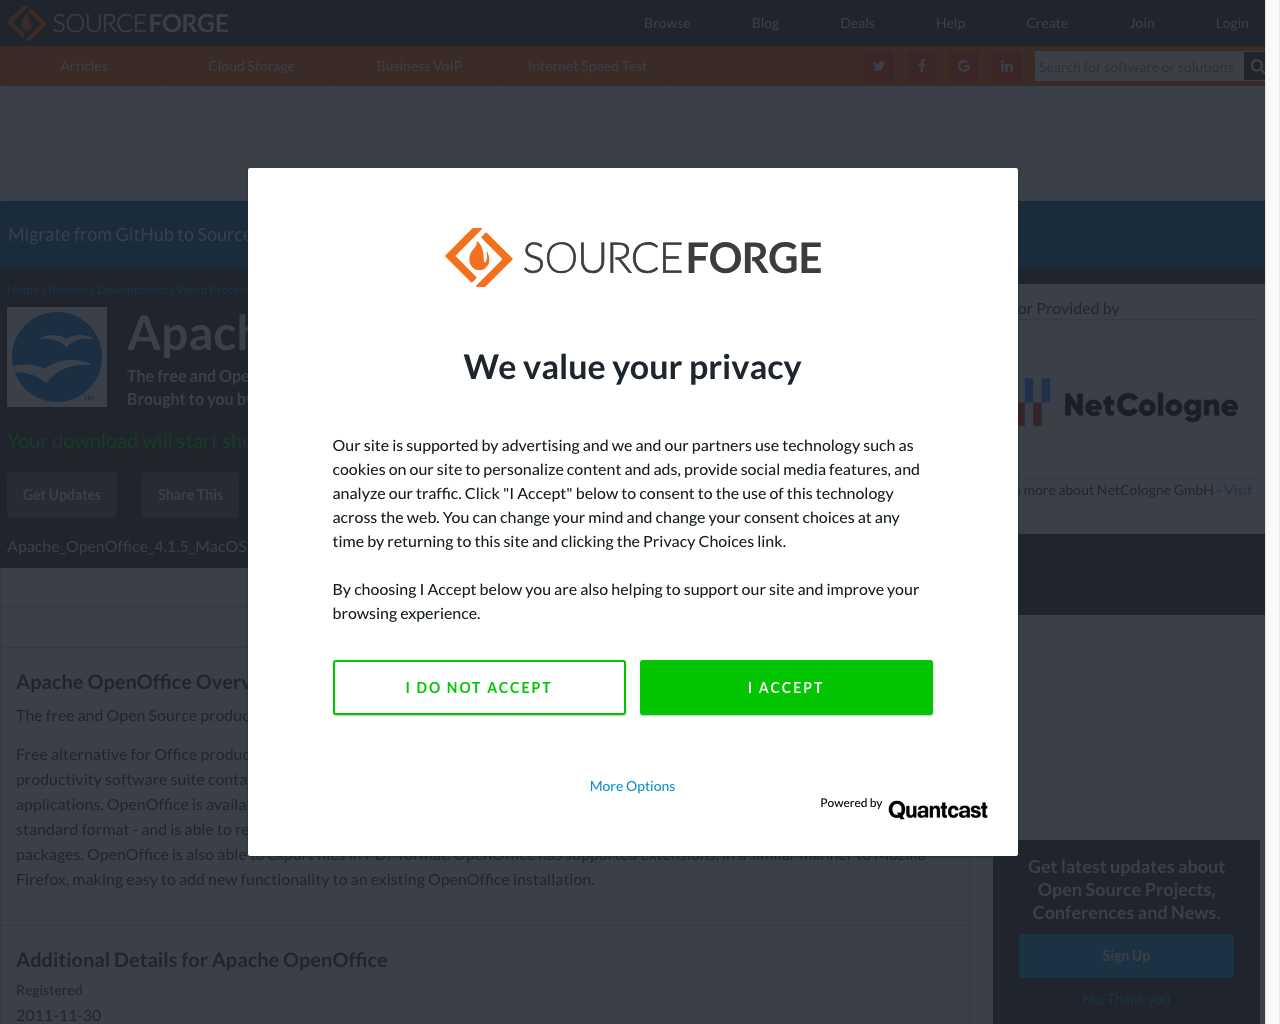
\includegraphics[width=1.0\linewidth]{pic0002}
  \caption{Съгласие с общите условия на SourceForge}
\label{figure0002}
\end{figure}
\FloatBarrier

Следва уеб страница за съгласие с общите условия SourceForge (Фиг. \ref{figure0002}), където се съхраняват бинарните инсталационни файлове на продукта.

\begin{figure}[h!]
  \centering
  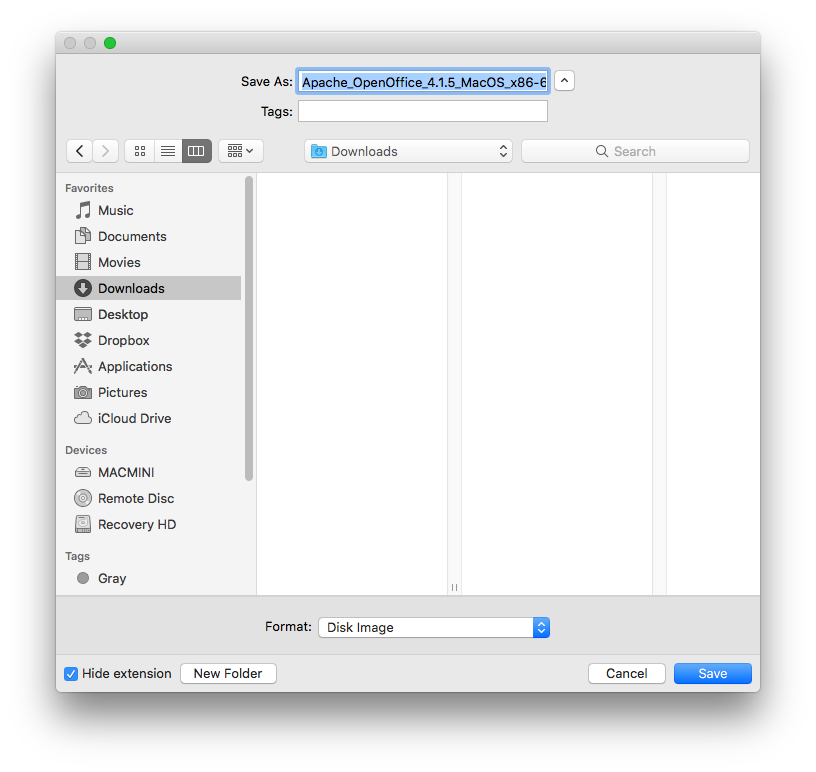
\includegraphics[width=1.0\linewidth]{pic0003}
  \caption{Запазване на инсталационния файл}
\label{figure0003}
\end{figure}
\FloatBarrier

След 5 секунди изчакване се появява диалогова кутия, която предлага възможност за съхраняване на инсталационния файл (Фиг. \ref{figure0003}).

\begin{figure}[h!]
  \centering
  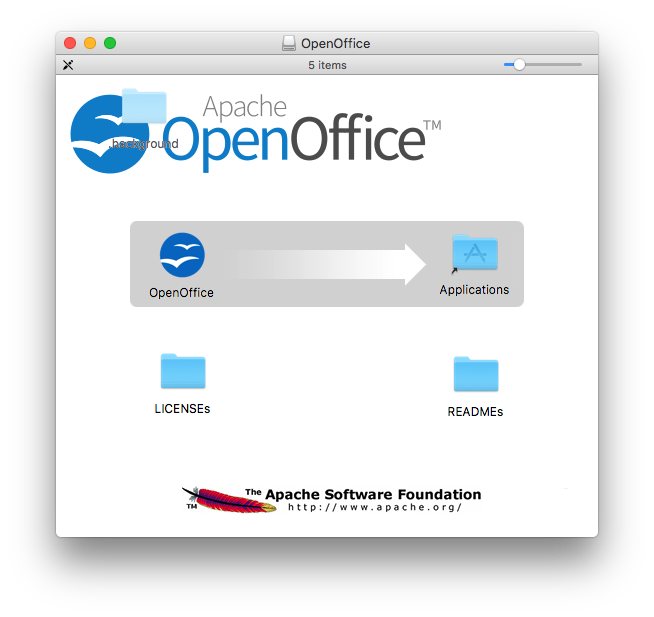
\includegraphics[width=1.0\linewidth]{pic0004}
  \caption{Стартиране на инсталатора}
\label{figure0004}
\end{figure}
\FloatBarrier

Двойно кликване с левия бутон на мишката върху файла на инсталатора води до неговото стартиране (Фиг. \ref{figure0004}).

\begin{figure}[h!]
  \centering
  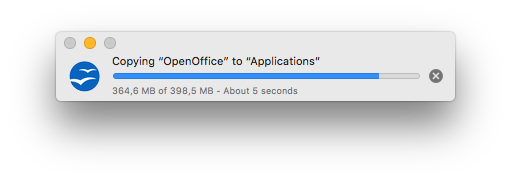
\includegraphics[width=1.0\linewidth]{pic0005}
  \caption{Процес за инсталация}
\label{figure0005}
\end{figure}
\FloatBarrier

Инсталацията\index{инсталация на продукта} основно протича с копиране на файловете в избраната директория за приложения (Фиг. \ref{figure0005}).

\section{Стартиране}

\begin{figure}[h!]
  \centering
  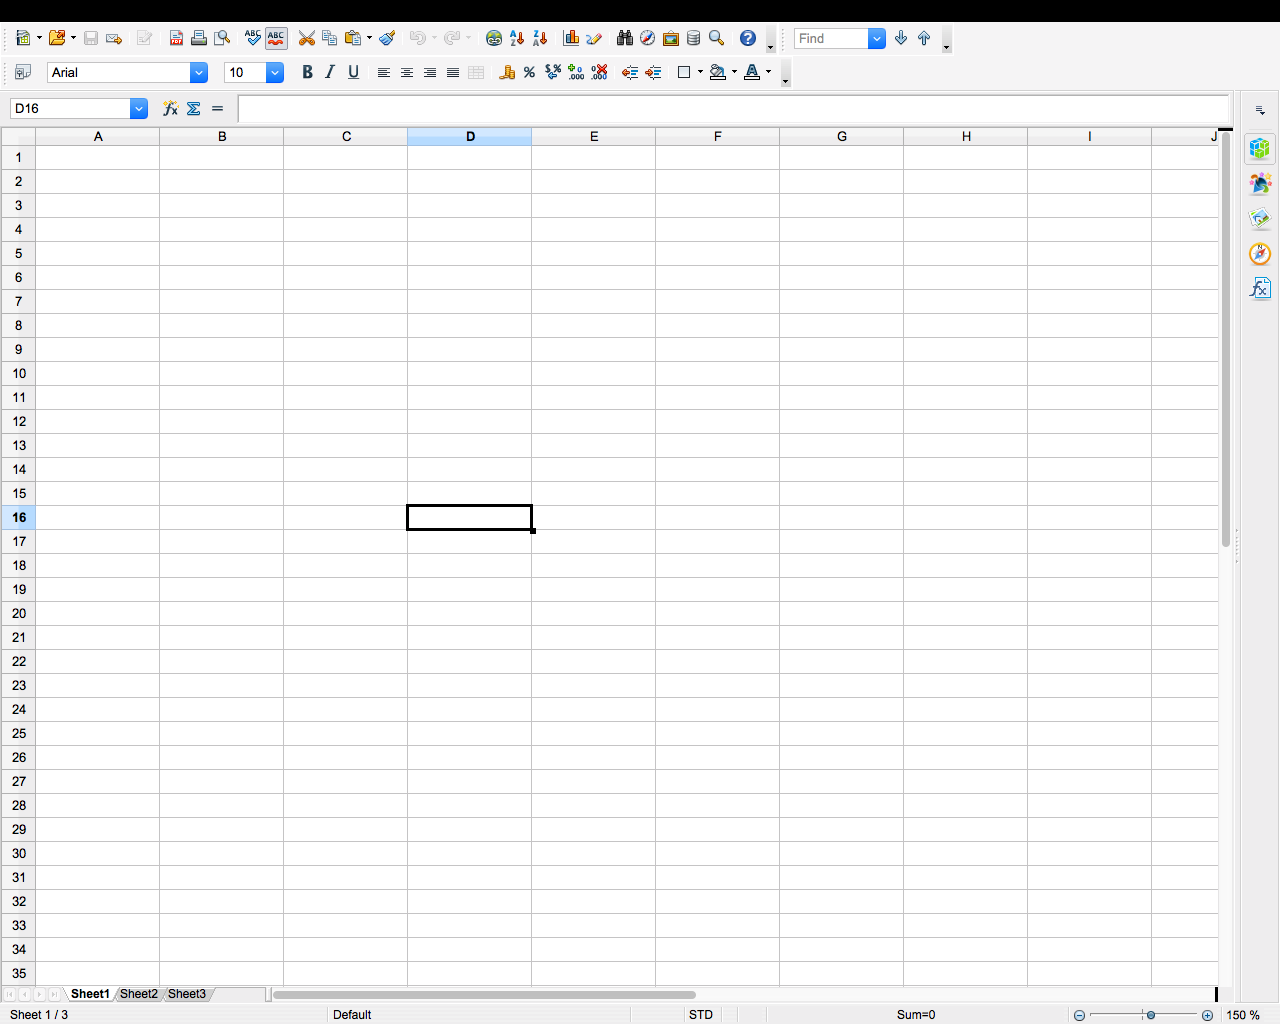
\includegraphics[width=1.0\linewidth]{pic0006}
  \caption{Основен прозорец на Apache OpenOffice Calc}
\label{figure0006}
\end{figure}
\FloatBarrier

След успешна инсталация, през икона за OpenOffice, след стартиране\index{стартиране на продукта} на Calc основният прозорец има изгледът от Фиг. \ref{figure0006}.

Работата с OpenOffice има следните предимства, спрямо алтернативни софтуерни продукти:

* Може да се използва без заплащане на лицензионна такса;

* Може да се използва на всички популярни операционни системи (Windows, Mac OS X, Linux); 

* Интерфейсът е достъпен на повече от 40 езика, като за повече от 70 езика има инструменти за проверка на правописа, сричкопренасяне и речници с думи;

* Поддържат се множество файлови формати, като е възможно експортиране в PDF и работа с Microsoft Office файловите формати. 

